%-----------------------------------------------------------------------------------------------------------------------------------------------%
%	The MIT License (MIT)
%
%	Copyright (c) 2015 DUVEY Maxime
%
%	Permission is hereby granted, free of charge, to any person obtaining a copy
%	of this software and associated documentation files (the "Software"), to deal
%	in the Software without restriction, including without limitation the rights
%	to use, copy, modify, merge, publish, distribute, sublicense, and/or sell
%	copies of the Software, and to permit persons to whom the Software is
%	furnished to do so, subject to the following conditions:
%	
%	THE SOFTWARE IS PROVIDED "AS IS", WITHOUT WARRANTY OF ANY KIND, EXPRESS OR
%	IMPLIED, INCLUDING BUT NOT LIMITED TO THE WARRANTIES OF MERCHANTABILITY,
%	FITNESS FOR A PARTICULAR PURPOSE AND NONINFRINGEMENT. IN NO EVENT SHALL THE
%	AUTHORS OR COPYRIGHT HOLDERS BE LIABLE FOR ANY CLAIM, DAMAGES OR OTHER
%	LIABILITY, WHETHER IN AN ACTION OF CONTRACT, TORT OR OTHERWISE, ARISING FROM,
%	OUT OF OR IN CONNECTION WITH THE SOFTWARE OR THE USE OR OTHER DEALINGS IN
%	THE SOFTWARE.
%	
%
%-----------------------------------------------------------------------------------------------------------------------------------------------%

%Balise versionning
\newif\ifenglish
% Uncomment the next line to set the flag to true.
% \englishtrue


%----------------------------------------------------------------------------------------
%	VARIABLES
%----------------------------------------------------------------------------------------
\newcommand{\myemail}{maxime.duvey@outlook.com}
\newcommand{\phonenumber}{+33 648 34 40 56}


%============================================================================%
%
%	DOCUMENT DEFINITION
%
%============================================================================%

%we use article class because we want to fully customize the page and dont use a cv template
\documentclass[10pt,A4]{article}	


%----------------------------------------------------------------------------------------
%	ENCODING
%----------------------------------------------------------------------------------------

%we use utf8 since we want to build from any machine
\usepackage[utf8]{inputenc}		

%----------------------------------------------------------------------------------------
%	LOGIC
%----------------------------------------------------------------------------------------

% provides \isempty test
\usepackage{xifthen}

%----------------------------------------------------------------------------------------
%	FONT
%----------------------------------------------------------------------------------------

% some tex-live fonts - choose your own

%\usepackage[defaultsans]{droidsans}
%\usepackage[default]{comfortaa}
%\usepackage{cmbright}
\usepackage[default]{raleway}
%\usepackage{fetamont}
%\usepackage[default]{gillius}
%\usepackage[light,math]{iwona}
%\usepackage[thin]{roboto} 

% set font default
\renewcommand*\familydefault{\sfdefault} 	
\usepackage[T1]{fontenc}

% more font size definitions
\usepackage{moresize}		


%----------------------------------------------------------------------------------------
%	PAGE LAYOUT  DEFINITIONS
%----------------------------------------------------------------------------------------

%debug page outer frames
%\usepackage{showframe}			


%define page styles using geometry
\usepackage[a4paper]{geometry}		

% for example, change the margins to 2 inches all round
\geometry{top=1.75cm, bottom=-.6cm, left=1.5cm, right=1.5cm} 	

%use customized header
\usepackage{fancyhdr}				
\pagestyle{fancy}

%less space between header and content
\setlength{\headheight}{-5pt}		


%customize entries left, center and right
\lhead{}
\ifenglish
\chead{ \small{DUVEY Maxime  $\cdot$ Software Engineer $\cdot$  Paris, France  $\cdot$  \textcolor{sectcol}{\textbf{\myemail}}  $\cdot$ \phonenumber}}
\else
\chead{ \small{DUVEY Maxime  $\cdot$ Ingénieur Logiciel $\cdot$  Paris, France  $\cdot$  \textcolor{sectcol}{\textbf{\myemail}}  $\cdot$ \phonenumber}}
\fi
\rhead{}


%indentation is zero
\setlength{\parindent}{0mm}

%----------------------------------------------------------------------------------------
%	TABLE /ARRAY DEFINITIONS
%---------------------------------------------------------------------------------------- 

%for layouting tables
\usepackage{multicol}			
\usepackage{multirow}

%extended aligning of tabular cells
\usepackage{array}

\newcolumntype{x}[1]{%
>{\raggedleft\hspace{0pt}}p{#1}}%


%----------------------------------------------------------------------------------------
%	GRAPHICS DEFINITIONS
%---------------------------------------------------------------------------------------- 

%for header image
\usepackage{graphicx}

%for floating figures
\usepackage{wrapfig}
\usepackage{float}
%\floatstyle{boxed} 
%\restylefloat{figure}

%for drawing graphics		
\usepackage{tikz}				
\usetikzlibrary{shapes, backgrounds,mindmap, trees}


%----------------------------------------------------------------------------------------
%	Color DEFINITIONS
%---------------------------------------------------------------------------------------- 

\usepackage{color}

%accent color
\definecolor{sectcol}{RGB}{255,150,0}

%dark background color
\definecolor{bgcol}{RGB}{110,110,110}

%light background / accent color
\definecolor{softcol}{RGB}{225,225,225}


%============================================================================%
%
%
%	DEFINITIONS
%
%
%============================================================================%

%----------------------------------------------------------------------------------------
% 	HEADER
%----------------------------------------------------------------------------------------

% remove top header line
\renewcommand{\headrulewidth}{0pt} 

%remove botttom header line
\renewcommand{\footrulewidth}{0pt}	  	

%remove pagenum
\renewcommand{\thepage}{}	

%remove section num		
\renewcommand{\thesection}{}			

%----------------------------------------------------------------------------------------
% 	ARROW GRAPHICS in Tikz
%----------------------------------------------------------------------------------------

% a six pointed arrow poiting to the left
\newcommand{\tzlarrow}{(0,0) -- (0.2,0) -- (0.3,0.2) -- (0.2,0.4) -- (0,0.4) -- (0.1,0.2) -- cycle;}	

% include the left arrow into a tikz picture
% param1: fill color
%
\newcommand{\larrow}[1]
{\begin{tikzpicture}[scale=0.58]
	 \filldraw[fill=#1!100,draw=#1!100!black]  \tzlarrow
 \end{tikzpicture}
}

% a six pointed arrow poiting to the right
\newcommand{\tzrarrow}{ (0,0.2) -- (0.1,0) -- (0.3,0) -- (0.2,0.2) -- (0.3,0.4) -- (0.1,0.4) -- cycle;}

% include the right arrow into a tikz picture
% param1: fill color
%
\newcommand{\rarrow}
{
\begin{tikzpicture}[scale=0.7]
	\filldraw[fill=sectcol!100,draw=sectcol!100!black] \tzrarrow
 \end{tikzpicture}
}



%----------------------------------------------------------------------------------------
%	custom sections
%----------------------------------------------------------------------------------------

% create a coloured box with arrow and title as cv section headline
% param 1: section title
%
\newcommand{\cvsection}[1]
{
\colorbox{sectcol}{\mystrut \makebox[1\linewidth][l]{
\larrow{bgcol} \hspace{-8pt} \larrow{bgcol} \hspace{-8pt} \larrow{bgcol} \textcolor{white}{\textbf{#1}}\hspace{4pt}
}}\\
}

%create a coloured arrow with title as cv meta section section
% param 1: meta section title
%
\newcommand{\metasection}[2]
{
\begin{tabular*}{1\textwidth}{p{2.4cm} p{11cm}}
\larrow{bgcol}	\normalsize{\textcolor{sectcol}{#1}}&#2\\[12pt]
\end{tabular*}
}

\newcommand{\newmetasection}[2]
{
\begin{tabular*}{1\textwidth}{p{2.4cm} p{15cm}}
\larrow{bgcol}	\normalsize{\textcolor{sectcol}{#1}}&#2\\[12pt]
\end{tabular*}
}

%----------------------------------------------------------------------------------------
%	 CV EVENT
%----------------------------------------------------------------------------------------

% creates a stretched box as cv entry headline followed by two paragraphs about 
% the work you did
% param 1:	event time i.e. 2014 or 2011-2014 etc.
% param 2:	event name (what did you do?)
% param 3:	institution (where did you work / study)
% param 4:	what was your position
% param 5:	some words about your contributions
%
\newcommand{\cvevent}[5]
{
\vspace{8pt}
	\begin{tabular*}{1\textwidth}{p{2.3cm}  p{10.8cm} x{3.9cm}}
 \textcolor{bgcol}{#1}& \textbf{#2} & \vspace{2.5pt}\textcolor{sectcol}{#3}

	\end{tabular*}
\vspace{-12pt}
\textcolor{softcol}{\hrule}
\vspace{6pt}
	\begin{tabular*}{1\textwidth}{p{2.3cm} p{14.4cm}}
&		 \larrow{bgcol}  #4\\[3pt]
&		 \larrow{bgcol}  #5\\[6pt]
	\end{tabular*}

}

% creates a stretched box as 
\newcommand{\cveventmeta}[2]
{
	\mbox{\mystrut \hspace{87pt}\textit{#1}}\\
	#2
}

%----------------------------------------------------------------------------------------
% CUSTOM STRUT FOR EMPTY BOXES
%----------------------------------------- -----------------------------------------------
\newcommand{\mystrut}{\rule[-.3\baselineskip]{0pt}{\baselineskip}}

%----------------------------------------------------------------------------------------
% CUSTOM LOREM IPSUM
%----------------------------------------------------------------------------------------
\newcommand{\lorem}
{}



%============================================================================%
%
%
%
%	DOCUMENT CONTENT
%
%
%
%============================================================================%
\begin{document}


%use our custom fancy header definitions
\pagestyle{fancy}	


%---------------------------------------------------------------------------------------
%	TITLE HEADLINE
%----------------------------------------------------------------------------------------
\vspace{-20.55pt}

% use this for multiple words like working titles etc.
%\hspace{-0.25\linewidth}\colorbox{bgcol}{\makebox[1.5\linewidth][c]{\hspace{46pt}\HUGE{\textcolor{white}{\textsc{DUVEY Maxime}} } \textcolor{sectcol}{\rule[-1mm]{1mm}{0.9cm}} \parbox[b]{5cm}{   \large{ \textcolor{white}{{IT Consultant}}}\\
% \large{ \textcolor{white}{{Resume}}}}
%}}

% use this for single words, e.g. CV or RESUME etc.
\hspace{-0.25\linewidth}\colorbox{bgcol}{\makebox[1.5\linewidth][c]{\HUGE{\textcolor{white}{\textsc{DUVEY Maxime}} } \textcolor{sectcol}{\rule[-1mm]{1mm}{0.9cm}} \HUGE{\textcolor{white}{\textsc{Resume}} } }}


%----------------------------------------------------------------------------------------
%	HEADER IMAGE
%----------------------------------------------------------------------------------------

\begin{figure}[H]
\begin{flushright}
	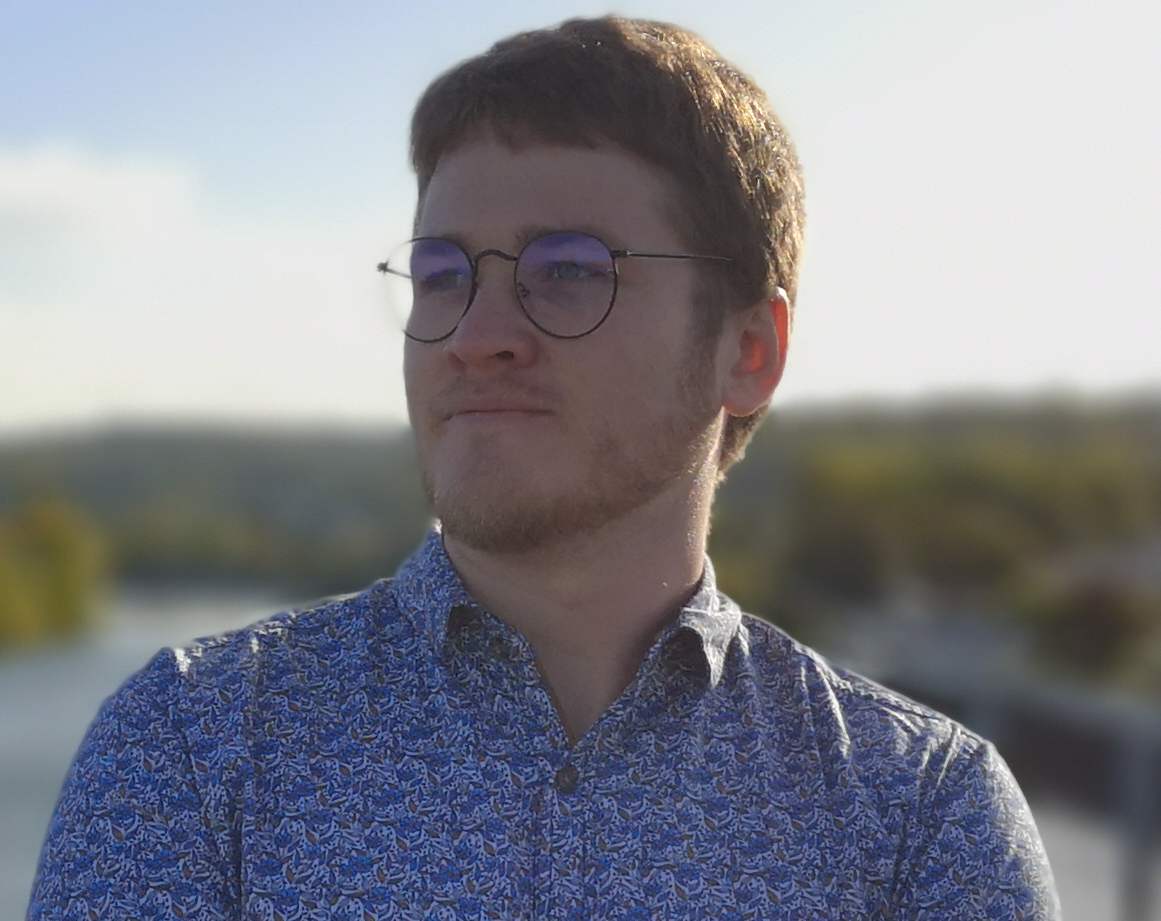
\includegraphics[clip,width=0.2\linewidth]{newphoto.png}	%trimming relative to image size!
\end{flushright}
\end{figure}

%---------------------------------------------------------------------------------------
%	QR CODE (optional)
%----------------------------------------------------------------------------------------
%\vspace{-136pt}
%\hspace{0.75\linewidth}
%
\includegraphics[width=103pt]{qrcode}
%\normalsize
%\vspace{88pt}

%---------------------------------------------------------------------------------------
%	META SECTION
%----------------------------------------------------------------------------------------

\vspace{-114pt}

\ifenglish
\metasection{Status:}{Freelance disponible a partir:  \textbf{ 1 Février 2024}}
\metasection{Fields:}{Developement Logiciel, et systemes embarqués} 
\metasection{Tech:}{C++,  C, java, Kotlin, linux, AOSP}
\metasection{Interests:}{Robotique (Modélisation, Conception, Programation), informatique en général, science fiction }
\else
\metasection{Status:}{Freelance available: \textbf{ 1 February 2024 } }
\metasection{Fields:}{Software and Embedded System Engineer} 
\metasection{Tech:}{C++,  C, java, Kotlin, linux, AOSP}
\metasection{Interests:}{Robotics (Modeling, Design, Programming), computer science in general, science fiction }
\fi

\vspace{6pt}

%---------------------------------------------------------------------------------------
%	SUMMARAY (optional)
%----------------------------------------------------------------------------------------

%\cvsection{Summary}\\
%I am a digital media graduate (M.Sc.) with project experience in educational research as well as in the private sector. During my studies I focused on e-assessment software and moved over to b2b software for IBM Notes Domino.

%Currently I develop and evaluate the next generation learning management system with Meteor based on an extensive nursing curriculum for healthcare education.  I also love fitness, martial arts, videogames, news and Sci-Fi series.\\[-2pt]

%============================================================================%
%
%	CV SECTIONS AND EVENTS (MAIN CONTENT)
%
%============================================================================%

%---------------------------------------------------------------------------------------
%	EXPERIENCE
%----------------------------------------------------------------------------------------
\cvsection{Experience}

% Sagemcom
\ifenglish
 \cvevent{Since 09/2022}{Software and Embedded System Engineer}{Sagemcom}{Software and embedded systems (Linux and AOSP) development in the field of telecommunications and entertainment.}{Linux, Android, Android-studio, C++, C, Java, Kotlin, AOSP}
\else
\cvevent{Depuis 09/2022-}{Ingénieur logiciel et systeme embarqué}{Sagemcom}{Développement logiciel et système embarqué dans le domaine de télécomunication et du divertissement.}{Linux, Android, Android-studio, C++, C, Java, Kotlin, AOSP}
\fi
%\textcolor{softcol}{\hrule}

% SII - mbda
\ifenglish
\cvevent{07/2021-09/2022}{Software development on embedded systems}{SII}{Software development on embedded systems for aerospace and military company.}{C++ , eclipse, DDS, UDP, Design Patterns, MISRA, Linux}
\else
\cvevent{ 07/2021-09/2022}{Ingénieur logiciel sur systèmes embarqués}{SII}{Développement logiciel sur système embarqué dans le domaine de l'aérospatial et de la défense.}{C++ , eclipse, DDS, UDP, Design Patterns, MISRA, Linux}
\fi
%\textcolor{softcol}{\hrule}

% ALTEN
\ifenglish
\cvevent{12/2018 - 2021}{Software development}{ALTEN}{Maintenance and improvement of network coverage optimization software (wave propagation), then interfacing C++ - C\#  for calculator with implementation of a license manager}{C\#, CLI, C++, Visual Studio, Jenkins, Design Patterns}
\else
\cvevent{12/2018 - 2021}{Ingénieur logiciel}{ALTEN}{Maintien et amélioration d'un logiciel d'optimisation de couverture réseau (propagation d'ondes), puis Interfacage C++ - C\# pour calculateur avec mise en place d'un gestionnaire de licence.}{C\#, CLI, C++, Visual Studio, Jenkins, Design Patterns}
\fi

%\textcolor{softcol}{\hrule}

% Bouygues Construction
\ifenglish
\cvevent{04/2018 - 10/2018}{Unity/UE4 Developer for Open Innovation VR department}{ Bouygues Construction}{Software and application development necessary for business needs in the field of virtual reality}{C\#, unity, Kinect, Réalité virtuel}
\else
\cvevent{04/2018 - 10/2018}{Développeur Unity/UE4 département Open Innovation VR}{ Bouygues Construction}{Développement des applications nécessaires aux besoins de l’entreprise dans le domaine de la réalité virtuelle}{C\#, unity, Kinect, Réalité virtuel}
\fi

%\textcolor{softcol}{\hrule}

% Epitech EIP
\ifenglish
\cvevent{11/2015 - 3/2018}{EIP end-of-studies project (Front and Lore pole leader)}{EPITECH}{Innovative professional project, from a team of 7 people, FPS - RPG in virtual reality}{C++, EU4, HTC Vive}
\else
\cvevent{11/2015 - 3/2018}{Projet de fin d'études EIP (chef pole Front et Lore)}{EPITECH}{Projet professionnel innovant, d'une équipe de 7 personnes, FPS - RPG en réalité virtuel}{C++, EU4, HTC Vive}
\fi

%\textcolor{softcol}{\hrule}

%
\ifenglish
\cvevent{2 * 1 month}{ASSET (assistant professor for C, PHP, Python, Ruby, Shell)}{ETNA}{Supervising Bachelors and Masters, our goal is to train students in programming languages during their swimming pools}{Called for the first time to supervise the bachelors, called back the following year for the Masters}
\else
\cvevent{2 * 1 mois}{ASSET (assistant professeur C, PHP, Python, Ruby, Shell)}{ETNA}{Encadrant des Bachelors et Master, notre but et de former les élèves sur des langages de programmation durant leurs piscines}{Appelée une première fois pour encadrer les bachelors, rappelé l'année suivante pour les Master}
\fi

%\textcolor{softcol}{\hrule}

%---------------------------------------------------------------------------------------
%	EDUCATION SECTION
%---------------------------------------------------------------------------------------
\cvsection{Education}

\cvevent{2013 - 2018}{Master's degree Software Engineering}{University of EPITECH}{Paris}{C - C++ - Linux}

\ifenglish
\cvevent{2016 - 2017}{4th year of study in China}{Jiaotong university}{Beijing}{Mainly C++ - Web - Linux}
\else
\cvevent{2016 - 2017}{4em année d'étude en Chine}{Jiaotong university}{Pékin}{Principalement  C++ - Web - Linux}
\fi

%\textcolor{softcol}{\hrule}

 

\newpage
%---------------------------------------------------------------------------------------
%	Annexe
%---------------------------------------------------------------------------------------
\cvsection{Annexe}

\ifenglish
\begin{center}{This part brings together the technologies and languages that I learned and used on my various personal projects.
Allowing a better representation of my profile and a better selection by CV parsers.}\end{center}
\else
\begin{center}{Cette partie regroupe les technologies et langages que j'ai appris et utilisés sur mes différents projets personnels.
Permettant une meilleure représentation de mon profil et une meilleure sélection par les parseurs de CV.}\end{center}
\fi

\vspace{6pt}
\newmetasection{Languages}{C++ (11<->17), C, C\#, Python(3), Java(Fx), Scripting, PHP, CSS, HTML, Ruby, Latex, XML, JSON, CSV, SQL, java, kotlin, }


\ifenglish

\vspace{10pt}
\newmetasection{Tools:}{Visual studio, Visual Code, Eclipse, Notepade++, Git, SVN, RTC, Symfony, wamp server, Arduino, PlatformIO, Jenkins, Cura, Freecad, UE4, GitKraken, Virtual Machine, Postman, Jira, Trello, wsl, cygwin, protobug, gRPC, AOSP (Android), vcpkg }

\vspace{10pt}
\newmetasection{Areas covered:}{Robotics (mechanical design, 3D modeling, 3D printing, electronics, PCB design, Embedded programming (on simple and complex environments), Creation of WEB sites, Implementation of Linux systems (Tails;) , Software programming in a very complex environment, implementation of a licensing system, creation of a mobile application, Pair-programming software programming, trading software (in progress), video stream processing.}
\else

\newmetasection{Outils:}{Visual studio, Visual Code, Eclipse, Notepade++, Git, SVN, RTC, Symfony, wamp server, Arduino, PlatformIO, Jenkins, Cura, Freecad, UE4, GitKraken, Virtual Machine, Postman, Jira, Trello, wsl, cygwin, protobug, gRPC, AOSP (Android), vcpkg }

\newmetasection{Domaines parcourues:}{Robotique (conception mécanique, modélisation 3D, Impression 3D, électronique, Conception de PCB, Programmation embarqué (sur environnement simple et complexe), Création de sites WEB, Mise en place de systèmes Linux (Tails ;), Programmation Logiciel sur environnement très complexe, mise en place de système de licensing, création d'application mobile, Programmation logiciel en pair-programming, logiciel de trading (en cours), traitement de flux vidéo.} 
\fi


\vspace{6pt}

%---------------------------------------------------------------------------------------
%	Langues
%--------------------------------------------------------------------------------------
\ifenglish
\cvsection{Languages}

\vspace{6pt}
\newmetasection{French}{first language}
\vspace{-6pt}
\newmetasection{English}{800 Toeic}
\vspace{-6pt}
\newmetasection{Japanese}{learning in progress}
\else
\cvsection{Langues}

\vspace{6pt}
\newmetasection{Francais}{Courant}
\vspace{-6pt}
\newmetasection{Anglais}{800 Toeic}
\vspace{-6pt}
\newmetasection{Japonais}{Notions - apprentissage en cours}
\fi




%-------------------------------------------------------------------------------------------------
%	ARTIFICIAL FOOTER (fancy footer cannot exceed linewidth) 
%--------------------------------------------------------------------------------------------------
\null
\vspace*{\fill}
\hspace{-0.25\linewidth}\colorbox{bgcol}{\makebox[1.5\linewidth][c]{\mystrut \small \textcolor{white}{DUVEY Maxime} $\cdot$ \textcolor{white}{\myemail  \phonenumber}}}




%============================================================================%
%
%
%
%	DOCUMENT END
%
%
%
%============================================================================%
\end{document}
